\chapter{Fast One-Ring Smoothing}
\label{chFONS}
In this chapter we present an updated version of the Fast One-Ring smoothing filter for scalar fields on discrete manifolds, based on the filter initially proposed by H. Mara and S. Krömker at the EUROGRAPHICS Workshop on Graphics and Cultural Heritage (2017) ~\cite[s.~3.2]{Mara17}. Since publication, further research has been conducted by the authors, and it was determined that improving the weighting methods was possible, therefore, modifcations to the algorithm were implemented directly within the GigaMesh \todoCitation{GigaMesh} framework. This chapter now presents the as-yet-unpublished version of the Fast One-Ring smoothing filter as it exists now, with more accuracte weighting based on the interpolation of function values to the center of gravity for each circular sector comprising the geodesic disc centered upon a vertex in a mesh.
%
%
%
%
%
\section{Points \& Edges}
\label{ch4sPE}
Given a point $\bp_0$ in a mesh $\bM$, which is comprised of $m$ number of vertices, the one-ring neighborhood $\bN$ can be defined as all the points $\bp_i$ which are adjacent to and share an edge with $\bp_0$, where $i \in \{1, \ldots, n\}$, with $n$ being the cardinality of $\bN$. The points in $\bN$ are always indexed in a clockwise direction\todoResearch{GigaMesh assumes a counter-clockwise direction}, yet may vary in value among vertices in $\bM$, however, the value must always be $\geq 2$, and though there is no upper limit, $n$ is typically $\leq 12$.%
\todoResearch{get real upper limit for n}.%
\todoBackground{define adjacent as sharing an edge in background}

The procedure for filtering a mesh begins by calculating the smallest edge length $\elm$ adjacent to the center point $\bp_0$, which be used later as the radius of a geodesic disc.\todoCitation{geodesic discs}
\begin{equation}
	\elm(\bp_0) := \text{min}^n_{i=1} (|\bp_i - \bp_0|)
	\label{eq:localMinimumEdgeLength}
\end{equation}%
\nomenclature[ba]{$\elm(\bp_v)$}{the smallest edge length in $\bN_v$}%

Furthermore, to ensure that the filter window remains the same size for all neighborhoods $\bN_v\;\forall v \in \{1,\ldots,m\}$, we define
\begin{equation}
	\gelm := \min\{\elm(\bp_0) \;|\; \bp_0 \in \bM\}
	\label{eq:globalMinimumEdgeLength}
\end{equation}%
\nomenclature[bb]{$\gelm$}{the smallest edge length in $\bM$}%
as the smallest edge length among all edges of the mesh $\bM$, and will then use this $\gelm$ in all the following computations in lieu of $\elm$.
%
Figure~\ref{fig:geodesicDisc} shows a typical configuration of a one-ring neighborhood with irregular faces, the geodesic disc $\bG$ with radius $\elm$, and the circular sectors $\bs_i$ to be used for weighting the function values of the face $\bt_i$.
\begin{figure}[ht]
\ffigbox
	{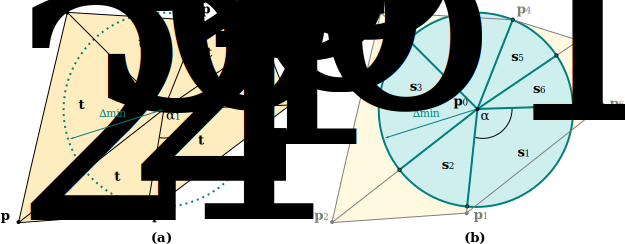
\includegraphics[width=1.0\linewidth]{figures/geodesicDisc.png}}
	{\caption[One-ring and geodesic disc]{A typical one-ring neighborhood $\bN$ with (a) irregular triangular faces $\bt_i$, the smallest edge length $\elm = |\bp_4 - \bp_0|$ shown here with a teal arrow as the radius of the geodesic disc, and $\alpha_i$ as the central angle of $\bt_i$ (b) the complete geodesic disc $\bG$, comprised of all its circular sectors $\bs_i$, each having central angles $\alpha_i$}\label{fig:geodesicDisc}}
\end{figure}%
\nomenclature[bc]{$\bG$}{the geodesic disc centered at $\bp_0$}%
\nomenclature[bd]{$\bs_i$}{the circle sectors which comprise $\bG$}%
%
%
%
%
%
\section{Angles}
\label{ch4sA}
In order to perform the many neccessary trigonometric operations required by the Fast One-Ring smoothing filter, we now compute the inner angles $\alpha_i$ of triangles $\bt_i$ using the using the Law of Cosines. \todoCitation{law of cosines}
\begin{equation}
	\alpha_i = cos^{-1}(\frac{|\bp_0 - \bp_{i}|^2 + |\bp_0 - \bp_{\sipo}|^2 - |\bp_i - \bp_{\sipo}|^2}{2\cdot|\bp_0 - \bp_{i}|\cdot|\bp_0 - \bp_{\sipo}|})
	\label{eq:alphaFromEdgeLengths}
\end{equation}%
\nomenclature[ca]{$\alpha_i$}{the central angle of $\bs_i$}%

We also require For interpolation of the function values over the entire circular sector, we must first interpolate the values one side of the bisecting line at a time. The angles $\beta_i$ are therefore calculated using the third angle theorem as the third angle to form a right triangle along with $\alpha_i\mathbin{/}2$ for each half of $\bs_i$. \todoCitation{and third angle theorems}
\begin{equation}
	\beta_i = \Big(\frac{\pi}{2} - \frac{\alpha_i}{2}\Big) = \frac{(\pi - \alpha_i)}{2}
	\label{eq:betaFromHalfAlpha}
\end{equation}%
\nomenclature[cb]{$\beta_i$}{the third angle with $\frac{\alpha_i}{2}$ and $\frac{\pi}{2}$}%
Figure~\ref{fig:angles} shows an example of the angles $\alpha_i$ and $\beta_i$ for the circle sector $\bs_i$  which comprises the geodesic disc $\bG$ with radius $\elm$.
\begin{figure}[ht]
\ffigbox
	{\includegraphics[width=0.8\linewidth]{example-image-16x9.png}}
	{\caption[The angles $\alpha_i$ and $\beta_i$]{An example of the angles $\alpha_i$ and $\beta_i$ for the circle sector $\bs_i$  which comprises the geodesic disc $\bG$ with radius $\elm$}\label{fig:angles}}
\end{figure}%
%
%
%
%
%
\section{Area \& Center of Gravity}
\label{ch4sACG}
We also need the area of each circular sector $\bs_i$ comprising the geodesic disc $\bG$, which can be calculated once both $\gelm$ and $\alpha_i$ have been determined
\begin{equation}
	A_i = \frac{(\gelm)^2\alpha_i}{2}
	\label{eq:circularSectorArea}
\end{equation}
\todoCitation{area of circle sectors, http://mathworld.wolfram.com/CircularSector.html}%
\nomenclature[da]{$A_i$}{area of circular sector $i$}%

Next, the distance from the center point $\bp_0$ to the center of gravity $\bc_i$ for the circular sector $\bs_i$ is calculated along the line which bisect the angle $\alpha_i$
\begin{equation}
	\Dc_i := \frac{2\:\gelm\:\sin(\frac{\alpha_i}{2})}{3\:\frac{\alpha_i}{2}}
	\label{eq:distToCoG}
\end{equation}
\todoCitation{area of circle sectors, http://mathworld.wolfram.com/CircularSector.html}%
\nomenclature[db]{$\Dc_i$}{the distance to $\bc_i$ within $\bs_i$}%

Figure~\ref{fig:centerOfGravity} illustrates the center of gravity $\bc_i$, or centroid, \todoCitation{centroid} and its distance from the center point $\bp_0$ of the circular sector $\bs_i$, using $\bs_1$ from Figure~\ref{eq:localMinimumEdgeLength} as an example. In general, the smaller the angle $\alpha_i$ becomes, the longer the distance $\Dc_1$ becomes.
\begin{figure}[ht]
\ffigbox
	{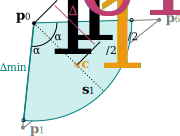
\includegraphics[width=0.6\linewidth]{figures/centerOfGravity.png}}
	{\caption[Distance to the Center of Gravity]{A single circle sector $\bs_1$ with a bisecting line in black dots and its center of gravity $\bc_1$ marked in a sand color, as well as the distance from the center point $\bp_0$ to $\bc_1$ drawn in coral as $\Dc_1$}\label{fig:centerOfGravity}}
\end{figure}%
\nomenclature[dc]{$\bc_i$}{the center of gravity, or centroid, of $\bs_i$}%
\todoReword{consider combining with angles figure}
\todoReword{lable ti}
%
%
%
%
%
%
\section{Interpolation \& Function Values}
\label{ch4sIFV}
\todoReword{add details about how function values come about}
With $\alpha_i\mathbin{/}2$, $\beta_i$, and $\gelm$ being constant for both halves of any circular sector $\bs_i$, we can next use the Law of Sines to obtain the constant ratio by which we will interpolate the three function values $f_0$, $f_i$, and $f_{\sipo}$ at the points $\bp_0$, $\bp_i$, and $\bp_{\sipo}$ which comprise the face $\bt_i$.
\begin{equation}
	\zeta_i = \frac{\gelm}{\sin(\beta_i)}
	\label{eq:zeta}
\end{equation}%
\nomenclature[ea]{$\zeta_i$}{constant ratio for interpolation derived from Law of Sines}%

With the constant ratio $\zeta_i$, we can obtain both of the distances required to interpolate $f_i$ and $f_{\sipo}$. It should be noted that because the points $\bp_i$ and $\bp_{\sipo}$ are likely at different distances from the center point $\bp_0$, we must now begin calculating for each half of the circular sector individually. One may look to Figures~\ref{fig:geodesicDisc} and~\ref{fig:centerOfGravity} for an example. Therefore, while subscript for $\zeta_i$ remains the match of index for the circle sector $\bs_i$, we will now adopt the subscipt for $\Dz_i$ to denote the side of the sector defined by its point $\bp_i$, also with $\Dz_{\sipo}$ for $\bp_{\sipo}$.
\begin{align}
	\Dz_i & = \kern4pt\frac{\zeta_i}{|\bp_0 - \bp_i|}
	\label{eq:distanceIForInterpolation}\\
	\Dz_{\sipo} & = \frac{\zeta_i}{|\bp_0 - \bp_{\sipo}|}
	\label{eq:distanceIp1ForInterpolation}
\end{align}%
\nomenclature[eb]{$\Dz^i_i$}{also $\Dz^i_{\sipo}$, the distances for interpolation of $f_i$ toward $f_0$}%

From the original function values $f_0$, $f_i$, and $f_{\sipo}$, we can now interpolate based on their distances $\Dz_i$ and $\Dz_{\sipo}$, to become
\begin{align}
	f'_i & = f_0(1 - \Dz_i) + f_i\Dz_i
	\label{eq:interpolatedFi} \\
	f'_{\sipo} & = f_0(1 - \Dz_{\sipo}) + f_{\sipo}\Dz_{\sipo}
	\label{eq:interpolatedFip1}
\end{align}%
\nomenclature[ec]{$f'_i$}{also $f'_{\sipo}$, the interpolated values of $f_i$ toward $f_0$}%

Figure~\ref{fig:interpolation} illustrates the\dots
\begin{figure}[ht]
\ffigbox
	{\includegraphics[width=0.6\linewidth]{example-image-16x9.png}}
	{\caption[Interpolation of Function Values toward the Centroid]{Interpolation of Function Values toward the Centroid\ldots}\label{fig:interpolation}}
\end{figure}
%
%
%
%
%
\section{Weighted Mean}
\label{ch4sWM}
To calculate the weighted mean function value $f^\bs_i$ at the center of gravity $\bc_i$ of the circle sector $\bs_i$, we must use $f_0$, the function value at $\bp_0$, both interpolated function values, $f'_i$ and $f'_{\sipo}$, and the distance to the center of gravity $\Dc_i$, and we obtain
\begin{equation}
	f^\bs_i = f_0(1 - \Dc_i) + \frac{(f'_i + f'_{\sipo})\Dc_i}{2}
	\label{eq:weightedMeanAtCoGatSector}
\end{equation}%
\nomenclature[fa]{$f^\bs_i$}{the weighted mean function value at $\bc_i$ of $\bs_i$}%

Finally, we can compute the one-ring weighted mean function value at $\bp_0$ by summing all the weighted mean function values from each $\bs_i$ in $\bN$, weighting those again by each sector's area $A_i$, then finally dividing by the total area of the geodesic disc.
\begin{equation}
	\bar{f}_0 := \frac{\sum A_if^{\bs}_i}{\sum A_i} \quad \forall i \in \{1,\ldots,|\bt_v|\}
	\label{eq:meanFuncValAtP0}
\end{equation}%
\nomenclature[fb]{$\bar{f}_0$}{the one-ring weighted mean function value at $\bp_0$}%

The one-ring smoothing filter can be modified to use the median operation, instead of the mean, by using all the equations except Equation~\ref{eq:meanFuncValAtP0} and then sorting the results of Equation~\ref{eq:weightedMeanAtCoGatSector}. The details of which can be found by the original publication ~\cite[s.~3.2]{Mara17}, but as it was not implemented in GPGPU for this thesis, we exclude the details here.

Figure~\ref{fig:weightedMean} illustrates the\dots
\begin{figure}[ht]
\ffigbox
	{\includegraphics[width=0.6\linewidth]{example-image-16x9.png}}
	{\caption[Weighted Mean function value $f^\bs_i$ at the center of gravity]{the weighted mean function value $f^\bs_i$ at the center of gravity\ldots 3D circle sector as base, floating plane above tilted be interpolated function values, area underneath colored.}\label{fig:weightedMean}}
\end{figure}
%
\section{Summary}
\label{ch4sS}
In this chapter we presented an updated version of the Fast One-Ring smoothing filter for scalar fields on discrete manifolds, which since its original publication ~\cite[s.~3.2]{Mara17}, now utilizes the entire area of the geodesic discs centered at $\bp_0$ to calculate the weighted averages of the function values in its one-ring neighborhood. First, we have illustrated how one can calculate the global smallest edge length $\gelm$, interior angles $\alpha$ and $\beta$, the area $A$ of a sector $\bs$ from the geodesic disc $\bG$, and distance $\Dc$ to the centroid (center of gravity) $\bc$ for any given one-ring neighborhood $\bN$ of mesh $\bM$. Next, we provided the equations for interpolating the three function values $f_0$, $f_i$, and $f_{\sipo}$ using the sectorially-constant ratio $\zeta$ to obtain the weighted mean function value for each $\bs$, and finally the weighted mean function value $\bar{f_0}$ at point ${\bp_0}$ for the entire one-ring neighborhood $\bN$. Convolving this filter with the scalar field of function values at each vertex in a mesh for any number of iterations, thus produces a smoothing effect with increasing intensity in relation to the number of iterations.
